\documentclass[11pt,a4paper]{article}

\usepackage[T1]{fontenc}
\usepackage[utf8]{inputenc}
\usepackage[english]{babel}
\usepackage[sc]{mathpazo}
\linespread{1.05}
\usepackage{microtype}
\usepackage[a4paper,margin=2.5cm]{geometry}
\usepackage{amsmath,amssymb,amsthm,mathtools}
\usepackage{graphicx}
\usepackage{booktabs,tabularx,array}
\usepackage{enumitem}
\usepackage[font=small,labelfont=bf,labelsep=colon]{caption}
\usepackage{xcolor}
\usepackage{tikz}
\usetikzlibrary{arrows.meta,calc,positioning,decorations.pathreplacing,fit,backgrounds}
\usepackage[most]{tcolorbox}
\usepackage{animate}
\usepackage[hidelinks]{hyperref}
% Floats go where they fit, so that few pages hold a float alone.
\makeatletter
\def\fps@figure{htbp}
\def\fps@table{htbp}
\makeatother
\renewcommand{\topfraction}{0.85}
\renewcommand{\bottomfraction}{0.6}
\renewcommand{\textfraction}{0.1}
\renewcommand{\floatpagefraction}{0.75}
\setcounter{topnumber}{3}
\setcounter{bottomnumber}{2}
\setcounter{totalnumber}{4}

% Phases as in the figures: climb green, search orange, transition blue; neutrals for text.
\definecolor{climb}{HTML}{1BAF7A}
\definecolor{search}{HTML}{EB6834}
\definecolor{transition}{HTML}{2A78D6}
\definecolor{ink}{HTML}{0B0B0B}
\definecolor{ink2}{HTML}{52514E}
\definecolor{muted}{HTML}{9A9893}
\definecolor{light}{HTML}{E6E5E1}

\tikzset{
  >={Stealth[length=1.8mm]},
  every picture/.style={line cap=round, line join=round},
  lbl/.style={font=\footnotesize},
  note/.style={font=\footnotesize, text=ink2},
  panel/.style={font=\small\bfseries, anchor=west},
  state/.style={circle, draw=#1, fill=#1!12, line width=1pt, minimum size=15mm, align=center, font=\small},
  box/.style={draw=ink2, fill=white, rounded corners=1.5pt, align=center, font=\small, inner sep=4pt},
}

\theoremstyle{definition}
\newtheorem{definition}{Definition}[section]
\theoremstyle{remark}
\newtheorem{remark}[definition]{Remark}

\newtcolorbox{inwords}{enhanced, breakable, colback=transition!5!white, colframe=transition, boxrule=0pt,
  leftrule=2.4pt, arc=0pt, outer arc=0pt, left=6pt, right=6pt, top=3pt, bottom=3pt,
  before upper={\textbf{In words.}\ }}
\newtcolorbox{keypoint}[1]{enhanced, breakable, colback=search!6!white, colframe=search, boxrule=0pt,
  leftrule=2.4pt, arc=0pt, outer arc=0pt, left=6pt, right=6pt, top=3pt, bottom=3pt,
  before upper={\textbf{#1}\par\smallskip}}

\newcommand{\st}[1]{\textsf{#1}}
\newcommand{\ind}{\mathbf{1}}
\newcommand{\cl}{\st{climb}}
\newcommand{\se}{\st{search}}
\newcommand{\tr}{\st{transition}}
% An animation written by plots.py; viewers that cannot play it show its last frame, the
% static figure.
\newcommand{\animated}[1]{\animategraphics[width=\textwidth,controls={play,step,stop},loop,poster=last,
  timeline=figures/#1_frames.tln]{8}{figures/#1_frames}{}{}}
\newcommand{\animmark}{\textcolor{transition}{$\blacktriangleright$}\ }

\title{\textbf{Flight phases with a hidden Markov model}\\[4pt]
  \large Vilpellet's labelling from scratch, what we keep,\\ and how far it reaches below 1~Hz}
\author{Matteo Di Sante}
\date{Method note, working version, 20 October 2026}

\begin{document}
\maketitle

\begin{abstract}
\noindent
Jérémie Vilpellet labels every fix of a soaring flight as \tr, \se\ or \cl\ with a three-state
hidden Markov model fed by three binary features: whether the track is straight, whether it rises,
and whether it turns one way~\cite{vilpellet2026,vilpellet2025}. This note explains the method from
scratch, for a reader who has never met a hidden Markov model; lists where his paper and his code
disagree; states what we keep and what we change to bring it into xc-dynamics; and measures how
far it reaches below 1~Hz. Every parameter of the method was fitted on 1-Hz tracks and counts
fixes, so a track logged every $\Delta$ seconds is first interpolated onto a 1-s grid. On 300
paraglider flights logged at 1~Hz and thinned to one fix every $\Delta$ seconds, the labels of the
full flight come back on 99.0\% of the kept fixes at $\Delta=2$~s and on 97.5\% at $\Delta=5$~s
when the interpolation is a cubic spline; linear interpolation loses one climbing fix in ten at
5~s, and at 10~s neither works.
\end{abstract}

\tableofcontents
\section*{The method at a glance}
\addcontentsline{toc}{section}{The method at a glance}

Figure~\ref{fig:overview} follows one segment of flight through the labelling;
Table~\ref{tab:glossary} gives each object in plain words. Figure~\ref{fig:window}, marked
\animmark, is animated: in Adobe Acrobat Reader, or another viewer that runs the JavaScript of PDF
files, the buttons below it play the animation; other viewers show the figure as printed. The note
answers four questions:
\begin{enumerate}[label=\arabic*.]
  \item \emph{How does the labelling work?} Sections~\ref{sec:hmm} (hidden Markov models, from
        zero) and~\ref{sec:method} (Vilpellet's method, step by step).
  \item \emph{Where do the paper and the code disagree?} Section~\ref{sec:conflicts}.
  \item \emph{What do we keep, and what do we change?} Section~\ref{sec:keep}.
  \item \emph{Can it label tracks logged every 2 or 5 seconds?} Section~\ref{sec:cadence}: yes, after
        a cubic-spline interpolation onto a 1-s grid; not every 10 seconds.
\end{enumerate}

\begin{figure}
\centering
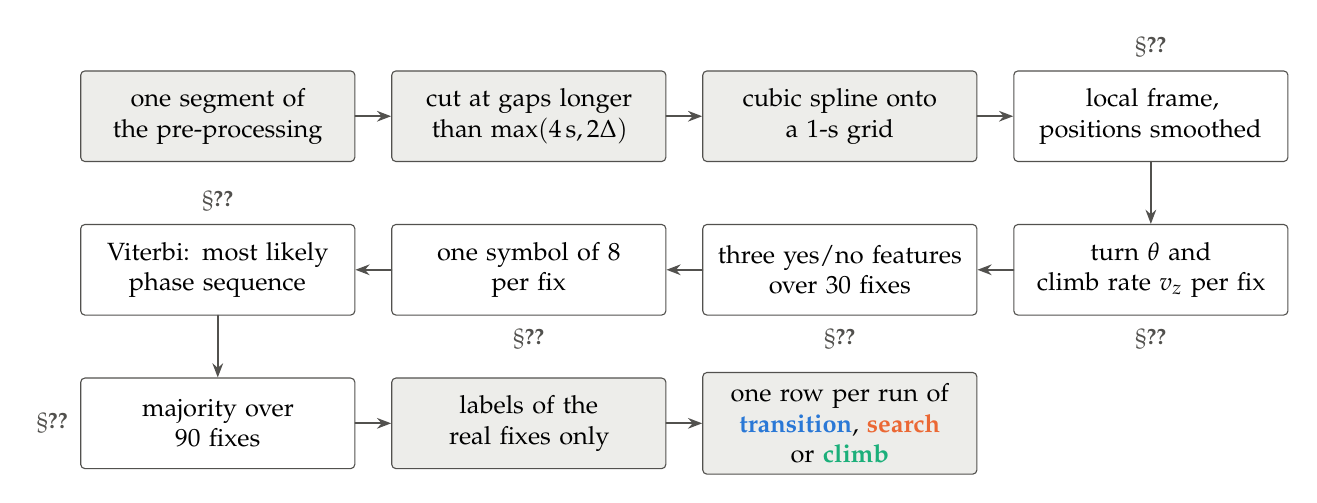
\begin{tikzpicture}[x=1cm,y=1cm, stage/.style={box, text width=3.2cm, minimum height=1.15cm},
    ours/.style={stage, fill=light!70}]
  \node[ours] (a) at (0,0) {one segment of\\the pre-processing};
  \node[ours] (b) at (3.95,0) {cut at gaps longer\\than $\max(4\,\mathrm{s},2\Delta)$};
  \node[ours] (c) at (7.9,0) {cubic spline onto\\a 1-s grid};
  \node[stage] (d) at (11.85,0) {local frame,\\positions smoothed};
  \node[stage] (e) at (11.85,-1.95) {turn $\theta$ and\\climb rate $v_z$ per fix};
  \node[stage] (f) at (7.9,-1.95) {three yes/no features\\over 30 fixes};
  \node[stage] (g) at (3.95,-1.95) {one symbol of 8\\per fix};
  \node[stage] (h) at (0,-1.95) {Viterbi: most likely\\phase sequence};
  \node[stage] (i) at (0,-3.9) {majority over\\90 fixes};
  \node[ours] (j) at (3.95,-3.9) {labels of the\\real fixes only};
  \node[ours] (k) at (7.9,-3.9) {one row per run of\\\textcolor{transition}{\textbf{transition}}, \textcolor{search}{\textbf{search}}\\or \textcolor{climb}{\textbf{climb}}};
  \foreach \u/\v in {a/b, b/c, c/d, d/e, e/f, f/g, g/h, h/i, i/j, j/k} \draw[->, ink2, line width=0.8pt] (\u) -- (\v);
  \node[note, above=1pt] at (d.north) {\S\ref{sec:frame}};
  \node[note, below=1pt] at (e.south) {\S\ref{sec:turn}};
  \node[note, below=1pt] at (f.south) {\S\ref{sec:features}};
  \node[note, below=1pt] at (g.south) {\S\ref{sec:emissions}};
  \node[note, above=1pt] at (h.north) {\S\ref{sec:three}};
  \node[note, left=1pt] at (i.west) {\S\ref{sec:decoding}};
\end{tikzpicture}
\caption{The labelling of one segment of flight. White: Vilpellet's method as his code runs it
(Section~\ref{sec:method}); grey: what xc-dynamics adds around it, the 1-s grid that lets coarser
loggers in (Section~\ref{sec:cadence}) and the storage (Section~\ref{sec:implementation}).}
\label{fig:overview}
\end{figure}

\begin{table}
\centering
\small
\begin{tabularx}{\textwidth}{@{}l X l@{}}
\toprule
Object & In words & Section \\
\midrule
fix & one recorded position; on the 1-s grid, one per second & \ref{sec:problem} \\
turn $\theta_k$ & how much the heading changes at fix $k$, in radians, positive to the left & \ref{sec:turn} \\
features $S,R,O$ & three yes/no answers about the 30 fixes around a fix: straight? rising? turning one way? & \ref{sec:features} \\
symbol & the three answers written as one number from 0 to 7 & \ref{sec:emissions} \\
state, phase & the hidden label of a fix: \cl, \se\ or \tr & \ref{sec:chain} \\
transition matrix $A$ & the probability of passing from one phase to another between two fixes & \ref{sec:chain} \\
emission $b_j(x)$ & the probability of seeing symbol $x$ while in phase $j$ & \ref{sec:hidden} \\
Viterbi path & the phase sequence with the highest probability given all the symbols & \ref{sec:three} \\
majority vote & each fix takes the phase most common in the 90 fixes around it & \ref{sec:decoding} \\
\bottomrule
\end{tabularx}
\caption{A minimal dictionary.}
\label{tab:glossary}
\end{table}

\section{The problem}\label{sec:problem}

A cross-country flight alternates three phases (Figure~\ref{fig:flight}), the
transition--search--climb cycle of~\cite{vilpellet2026}:
\begin{itemize}
  \item \textcolor{transition}{\textbf{transition}}: the pilot glides from one thermal towards the
        next; the track is nearly straight and sinks;
  \item \textcolor{search}{\textbf{search}}: there is no lift where the pilot expected it; the pilot
        turns, probes and changes heading; the track bends without a settled direction and the
        height changes little;
  \item \textcolor{climb}{\textbf{climb}}: in a thermal the pilot circles, always turning the same
        way, and rises.
\end{itemize}
Labelling every fix with its phase gives the statistics of each phase: how long climbs last, how
far glides go, how much time a pilot spends searching.

\begin{figure}
\centering
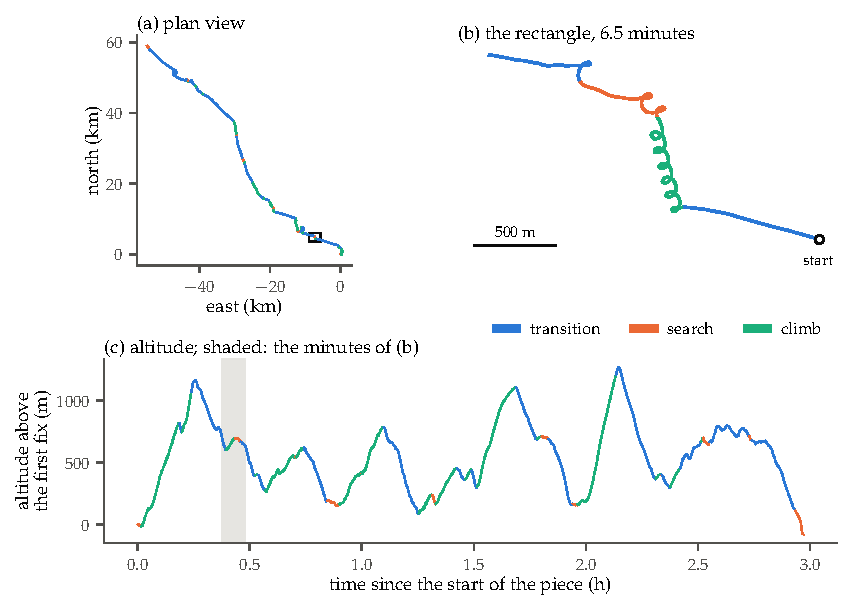
\includegraphics[width=\textwidth]{figures/flight_phases.pdf}
\caption{A 3-hour paraglider flight labelled by the method at 1~Hz. (a) Plan view; the rectangle
is panel (b). (b) 6.5 minutes of it: a glide, a climb that drifts with the wind, a search, and a
glide again. (c) GNSS altitude above the first fix of the piece: the climbs are the rising
stretches; the shaded band marks the minutes of (b), within the 24 minutes of
Figure~\ref{fig:features}.}
\label{fig:flight}
\end{figure}

Two things make the labelling hard. Nobody has labelled the fixes by hand, and the phases are only
partly objective: the end of a glide and the start of a search have no sharp boundary. And a GNSS
fix wobbles by a few metres, enough to fake a turn at one fix per second. Vilpellet answers both
in two stages: simple yes/no features computed over 30~s absorb the wobble, and a hidden Markov
model picks the phase sequence that best explains the features while making each change of phase
costly.

\paragraph{Logging intervals.} The model was fitted on tracks logged once per second. Table~\ref{tab:cadence}
shows how many flights of the archive are logged at another interval: one paraglider flight in
three, and seven hang-glider flights in ten. Section~\ref{sec:cadence} is about them.

\begin{table}
\centering
\small
\begin{tabular}{@{}l r *{7}{r}@{}}
\toprule
 & flights & 1~s & 2~s & 3~s & 4~s & 5~s & 10~s & other \\
\midrule
paragliders & 185\,321 & 69.6\% & 9.5\% & 5.1\% & 2.2\% & 9.7\% & 2.4\% & 1.5\% \\
hang gliders & 6\,536 & 30.4\% & 13.5\% & 9.6\% & 3.0\% & 26.6\% & 15.2\% & 1.7\% \\
\bottomrule
\end{tabular}
\caption{Logging interval of the FFVL flights that pass the altitude and speed rules of the
xc-dynamics pre-processing (column \texttt{sampling\_s} of
\texttt{derived/preprocessing/vertical/flights.csv}).}
\label{tab:cadence}
\end{table}

\section{Hidden Markov models from zero}\label{sec:hmm}

\subsection{A chain of phases}\label{sec:chain}

Number the fixes $k=1,2,\dots,K$ and call $Q_k$ the phase of fix $k$. Suppose for a moment that we
could see it. The simplest model of how phases follow each other is a \emph{Markov chain}: the
phase of the next fix depends only on the phase of the current one,
\begin{equation}\label{eq:markov}
  P(Q_{k+1}=j \mid Q_k=i,\ Q_{k-1},\dots,Q_1) = a_{ij}.
\end{equation}
The numbers $a_{ij}$ form the \emph{transition matrix} $A$. Row $i$ lists where phase $i$ goes
next, so each row sums to 1. The first phase is drawn from the \emph{initial distribution}
$\nu_j=P(Q_1=j)$. Vilpellet's chain, one step per second (Figure~\ref{fig:chain}), is
\begin{equation}\label{eq:A}
  A=\begin{pmatrix} 0.9896 & 0.0035 & 0.0069\\ 0.0067 & 0.9900 & 0.0033\\ 0.0010 & 0.0071 & 0.9919 \end{pmatrix}
  \qquad\text{(rows and columns: \cl, \se, \tr).}
\end{equation}

The diagonal says how sticky each phase is: a climb goes on to the next fix with probability
0.9896. A run of phase $i$ therefore lasts $n$ fixes with probability $a_{ii}^{\,n-1}(1-a_{ii})$, a
geometric law with mean $1/(1-a_{ii})$: 96~s for a climb, 100~s for a search, 123~s for a
transition. The chain has no memory of how long it has been in a phase: a climb that has lasted
ten minutes ends at the next fix with the same probability as one that has just begun.

\begin{figure}
\centering
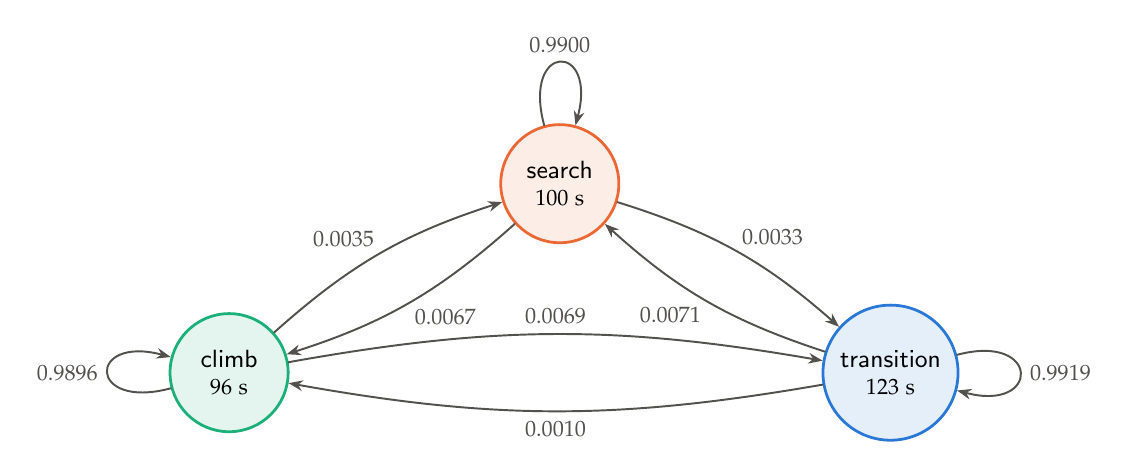
\begin{tikzpicture}[x=1cm,y=1cm, every loop/.style={min distance=11mm, looseness=6}]
  \node[state=climb] (C) at (0,0) {\cl\\[-1pt]{\footnotesize 96 s}};
  \node[state=search] (S) at (4.2,2.4) {\se\\[-1pt]{\footnotesize 100 s}};
  \node[state=transition] (T) at (8.4,0) {\tr\\[-1pt]{\footnotesize 123 s}};
  \path[->, ink2, line width=0.7pt, font=\footnotesize]
    (C) edge[loop left] node[left] {0.9896} (C)
    (S) edge[loop above] node[above] {0.9900} (S)
    (T) edge[loop right] node[right] {0.9919} (T)
    (C) edge[bend left=12] node[above left=-2pt] {0.0035} (S)
    (S) edge[bend left=12] node[below right=-2pt] {0.0067} (C)
    (C) edge[bend left=10] node[above] {0.0069} (T)
    (T) edge[bend left=10] node[below] {0.0010} (C)
    (S) edge[bend left=12] node[above right=-2pt] {0.0033} (T)
    (T) edge[bend left=12] node[below left=-2pt] {0.0071} (S);
\end{tikzpicture}
\caption{Vilpellet's chain of phases. Arrows carry the probability of the next fix's phase given the
current one; under each name, the mean duration $1/(1-a_{ii})$ seconds that the chain alone implies.}
\label{fig:chain}
\end{figure}

\begin{inwords}
$A$ is a table of habits: what usually follows what, one second at a time. It knows nothing about
the track.
\end{inwords}

\subsection{Hidden phases, visible symbols}\label{sec:hidden}

We never see $Q_k$. At each fix we see something else, $X_k$: in Vilpellet's method one of eight
symbols computed from the track (Section~\ref{sec:method}). Each phase produces the symbols with
its own probabilities, the \emph{emission probabilities}
\begin{equation}\label{eq:emission}
  b_j(x) = P(X_k=x \mid Q_k=j).
\end{equation}
The model assumes that once the phase of fix $k$ is known, its symbol depends on nothing else:
neither on the other phases nor on the other symbols. The probability of a phase sequence
$q_1,\dots,q_K$ together with the symbols $x_1,\dots,x_K$ is then a product of one factor per
fix (Figure~\ref{fig:graphical}):
\begin{equation}\label{eq:joint}
  P(q_{1:K},x_{1:K}) = \nu_{q_1}\,b_{q_1}(x_1)\prod_{k=2}^{K} a_{q_{k-1}q_k}\,b_{q_k}(x_k).
\end{equation}
This is a \emph{hidden Markov model} (HMM)~\cite{rabiner1989,zucchini2016}: a Markov chain that we
cannot see, observed through noisy symbols. Movement ecology labels the behaviour of animals from
GPS tracks with the same model, taking as observations the step length and the turning angle of
each fix, drawn from a law per state such as a gamma and a von
Mises~\cite{langrock2012,michelot2016}. Vilpellet's observations are of another kind: yes/no
summaries of 30 fixes of track, which Section~\ref{sec:assumptions} returns to.

\begin{figure}
\centering
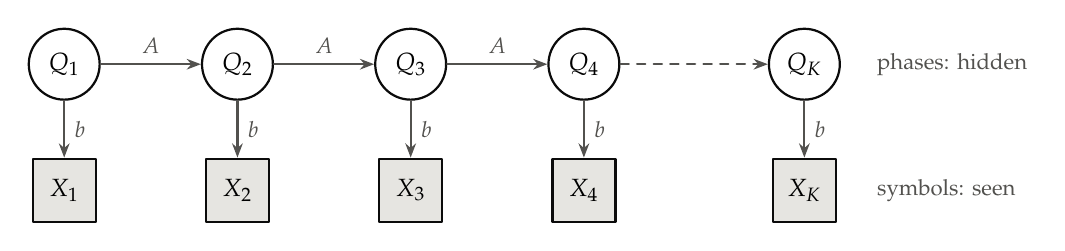
\begin{tikzpicture}[x=1cm,y=1cm,
    hid/.style={circle, draw=ink, line width=0.8pt, minimum size=9mm, font=\small},
    obs/.style={rectangle, draw=ink, fill=light, line width=0.8pt, minimum size=8mm, font=\small}]
  \foreach \k/\x in {1/0, 2/2.2, 3/4.4, 4/6.6} {
    \node[hid] (q\k) at (\x,1.6) {$Q_{\k}$};
    \node[obs] (x\k) at (\x,0) {$X_{\k}$};
    \draw[->, ink2, line width=0.8pt] (q\k) -- node[right, lbl] {$b$} (x\k);
  }
  \node[hid] (qK) at (9.4,1.6) {$Q_K$};
  \node[obs] (xK) at (9.4,0) {$X_K$};
  \draw[->, ink2, line width=0.8pt] (qK) -- node[right, lbl] {$b$} (xK);
  \foreach \a/\b in {q1/q2, q2/q3, q3/q4} \draw[->, ink2, line width=0.8pt] (\a) -- node[above, lbl] {$A$} (\b);
  \draw[->, ink2, line width=0.8pt, dashed] (q4) -- (qK);
  \node[note, anchor=west] at (10.2,1.6) {phases: hidden};
  \node[note, anchor=west] at (10.2,0) {symbols: seen};
\end{tikzpicture}
\caption{A hidden Markov model. Each phase depends only on the previous one, through $A$; each
symbol depends only on the phase of its own fix, through $b$.}
\label{fig:graphical}
\end{figure}

\subsection{A small example}\label{sec:toy}

Take two phases, climb $C$ and glide $G$, and one yes/no symbol: does the pilot rise (1) or sink
(0) at this step? Let both phases start with probability $0.5$, stay with probability $0.9$ and
switch with $0.1$, and let $b_C(1)=0.9$ and $b_G(1)=0.2$. The pilot shows
\[
  x = 1,\ 1,\ 0,\ 1,\ 1,\ 0,\ 0,\ 0 .
\]
Reading each symbol alone, the likelier phase is $C$ after a 1 and $G$ after a 0, which gives
$C\,C\,G\,C\,C\,G\,G\,G$: the single 0 at step 3 makes the pilot glide for one step. With the
chain, compare two sequences that differ only at step 3. By~\eqref{eq:joint} all their other
factors are equal, and
\[
  \frac{P(\dots C\,C\,C\dots)}{P(\dots C\,G\,C\dots)}
  = \frac{a_{CC}\,b_C(0)\,a_{CC}}{a_{CG}\,b_G(0)\,a_{GC}}
  = \frac{0.9\cdot0.1\cdot0.9}{0.1\cdot0.8\cdot0.1}\approx10 .
\]
Staying in the climb costs one unlikely symbol, $0.1$ instead of $0.8$; leaving and coming back
costs two unlikely changes, $0.1\times0.1$. The isolated sink is read as noise. The zeros from
step 6 on persist, and the best sequence switches to $G$ at step 6
(Figure~\ref{fig:trellis}). This is the job of the HMM in Vilpellet's method: a phase changes only
when the evidence persists.

\begin{figure}
\centering
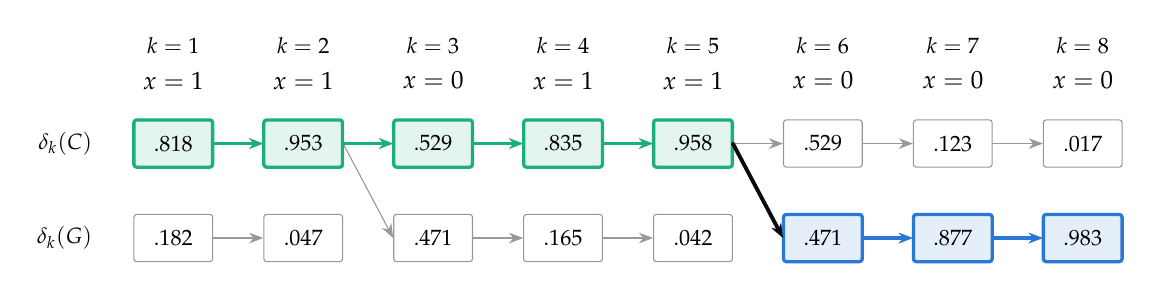
\begin{tikzpicture}[x=1.65cm,y=1cm,
    cell/.style={rectangle, draw=muted, rounded corners=1pt, minimum width=1.0cm, minimum height=0.6cm, font=\footnotesize, fill=white}]
  \foreach \k/\ob/\vc/\vg in {1/1/.818/.182, 2/1/.953/.047, 3/0/.529/.471, 4/1/.835/.165,
                              5/1/.958/.042, 6/0/.529/.471, 7/0/.123/.877, 8/0/.017/.983} {
    \node[lbl] at (\k,2.05) {$k=\k$};
    \node[font=\small\bfseries] at (\k,1.6) {$x=\ob$};
    \node[cell] (c\k) at (\k,0.8) {\vc};
    \node[cell] (g\k) at (\k,-0.4) {\vg};
  }
  \node[lbl, anchor=east] at (0.45,0.8) {$\delta_k(C)$};
  \node[lbl, anchor=east] at (0.45,-0.4) {$\delta_k(G)$};
  \foreach \k/\pc/\pg in {2/0/1, 3/0/0, 4/0/1, 5/0/1, 6/0/0, 7/0/1, 8/0/1} {
    \pgfmathtruncatemacro{\j}{\k-1}
    \ifnum\pc=0 \draw[->, muted] (c\j.east) -- (c\k.west); \else \draw[->, muted] (g\j.east) -- (c\k.west); \fi
    \ifnum\pg=0 \draw[->, muted] (c\j.east) -- (g\k.west); \else \draw[->, muted] (g\j.east) -- (g\k.west); \fi
  }
  \foreach \k in {1,...,5} \node[cell, draw=climb, line width=1.2pt, fill=climb!12] at (c\k) {};
  \foreach \k/\v in {1/.818, 2/.953, 3/.529, 4/.835, 5/.958} \node[font=\footnotesize] at (c\k) {\v};
  \foreach \k in {6,7,8} \node[cell, draw=transition, line width=1.2pt, fill=transition!12] at (g\k) {};
  \foreach \k/\v in {6/.471, 7/.877, 8/.983} \node[font=\footnotesize] at (g\k) {\v};
  \foreach \a/\b in {c1/c2, c2/c3, c3/c4, c4/c5} \draw[->, climb, line width=1.4pt] (\a.east) -- (\b.west);
  \draw[->, ink, line width=1.4pt] (c5.east) -- (g6.west);
  \foreach \a/\b in {g6/g7, g7/g8} \draw[->, transition, line width=1.4pt] (\a.east) -- (\b.west);
\end{tikzpicture}
\caption{Viterbi on the small example. Each cell holds $\delta_k(j)$, the probability of the best
sequence ending in phase $j$ at step $k$, divided by the sum of the column; the grey arrow into each
cell comes from its best predecessor. Steps 3 and 6 have the same scores, yet the path stays in $C$
at step 3 and leaves it at step 6: the decision depends on the symbols that follow, which is why
Viterbi reads the whole sequence before deciding.}
\label{fig:trellis}
\end{figure}

\subsection{Decoding and fitting}\label{sec:three}

\paragraph{The best phase sequence (Viterbi).} Write $\delta_k(j)$ for the highest
probability~\eqref{eq:joint} of any phase sequence of the first $k$ fixes that ends in phase $j$.
The best sequence ending in $j$ at fix $k$ comes from the best sequence ending in some $i$ at fix
$k-1$, so
\begin{equation}\label{eq:viterbi}
  \delta_1(j)=\nu_j\,b_j(x_1),\qquad
  \delta_k(j)=\max_i\bigl[\delta_{k-1}(i)\,a_{ij}\bigr]\,b_j(x_k),\qquad
  \psi_k(j)=\arg\max_i\bigl[\delta_{k-1}(i)\,a_{ij}\bigr].
\end{equation}
At the last fix one takes the best phase and follows the pointers $\psi$ backwards~\cite{viterbi1967,forney1973}.
The cost is $K\times S^2$ operations for $S$ phases, against the $S^K$ sequences one would
otherwise compare. The scores shrink at every fix and fall below the smallest number a computer
holds after a few hundred fixes; dividing the column by its sum at each fix, as Vilpellet's code
does, or working with logarithms, keeps them finite and leaves the path unchanged.

\paragraph{The parameters (Baum--Welch).} When $A$, $\nu$ and $b$ are unknown they are fitted by
expectation--maximisation~\cite{baum1970,rabiner1989}. Replacing the maximum of~\eqref{eq:viterbi}
by a sum, a forward and a backward pass give, under the current parameters, the probability
$\gamma_k(j)$ of each phase at each fix and the probability $\xi_k(i,j)$ of each change between
consecutive fixes, given all the symbols. Each round then re-estimates the parameters as expected
counts:
\begin{equation}\label{eq:baumwelch}
  \nu_j=\gamma_1(j),\qquad
  a_{ij}=\frac{\sum_k\xi_k(i,j)}{\sum_k\gamma_k(i)},\qquad
  b_j(x)=\frac{\sum_{k:\,x_k=x}\gamma_k(j)}{\sum_k\gamma_k(j)} .
\end{equation}
No round lowers the probability of the data, and the rounds stop at a local maximum, so the
starting guess matters. The middle formula is the update of $A$ that Vilpellet's training code
leaves out (Section~\ref{sec:conflicts}). The names of the states are not learnt: a state is
``climb'' only because its emissions look like a climb.

\begin{inwords}
Viterbi finds the best phase sequence; Baum--Welch fits the parameters by alternating ``guess the
phases softly'' and ``count''.
\end{inwords}

\subsection{What the model assumes}\label{sec:assumptions}

Three assumptions: phases have no memory, so their durations are geometric; symbols are
independent once the phases are known; the same parameters hold at every fix of every flight.
Vilpellet's symbols are computed over 30-s windows, so two consecutive symbols share 29 of their
30 fixes and are far from independent: the model counts the same evidence about thirty times. The
paper accepts this as approximately true at the scale of 30~s~\cite{vilpellet2026}. In practice
the windows carry the persistence and the HMM settles the changes of phase. None of the
probabilities the model computes is calibrated; only the labels are used.

\section{Vilpellet's method, step by step}\label{sec:method}

This section follows his reference inference script~\cite{vilpellet2025code}, which our rewrite
in \texttt{phases.py} reproduces bit for bit: features, Viterbi path and final labels coincide on
three real flights (\texttt{test\_note.py}). Every window counts fixes; on a 1-Hz track a fix is a
second.

\subsection{Local frame and smoothing}\label{sec:frame}

The method works on one piece of flight at a time, fixes in order. Latitude, longitude and GNSS
height become east, north and up coordinates $(e_k,n_k,u_k)$ in metres, in a frame tangent to the
Earth at the first fix of the piece (WGS84). Each coordinate is then smoothed with Gaussian
weights over six consecutive fixes, $k-3$ to $k+2$, with a standard deviation of one fix; the first
three and the last two fixes of a piece have no smoothed value. The third coordinate is the height
above the plane tangent at the first fix, which falls below the altitude by about $d^2/2R$ at a
distance $d$ from that fix: 785~m at 100~km. Its rate of change is the climb rate minus
$(d/R)\,\dot d$, with $\dot d$ the speed away from the first fix: 0.16~m/s less for a glide at
10~m/s, 100~km out (Section~\ref{sec:keep}).

\subsection{Turn and climb rate}\label{sec:turn}

The heading of the step from fix $k$ to fix $k+1$ is $\varphi_k=\operatorname{atan2}(n_{k+1}-n_k,\
e_{k+1}-e_k)$, and the \emph{turn} at fix $k$ is the change of heading, brought into $[-\pi,\pi)$
(Figure~\ref{fig:turn}):
\begin{equation}\label{eq:turn}
  \theta_k = \bigl((\varphi_k-\varphi_{k-1}+\pi) \bmod 2\pi\bigr)-\pi ,
\end{equation}
positive when the pilot turns left, anticlockwise seen from above. The turn is then averaged over
six fixes, $k-3$ to $k+2$. The code calls it \texttt{radius\_curvature} and the paper a curvature
angle; it is an angle per fix. A pilot circling once in 26~s turns by
$2\pi/26\approx0.24$~rad per fix. The climb rate is $v_{z,k}=(u_k-u_{k-1})/(t_k-t_{k-1})$, on the
smoothed height.

\begin{figure}
\centering
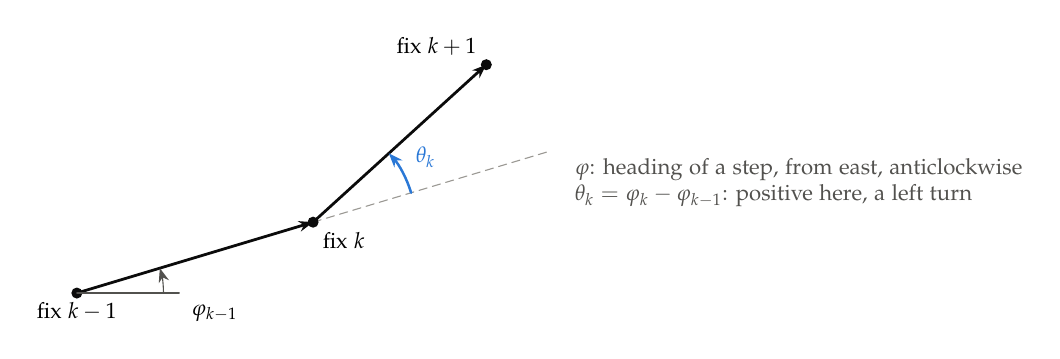
\begin{tikzpicture}[x=1cm,y=1cm]
  \coordinate (a) at (0,0); \coordinate (b) at (3,0.9); \coordinate (c) at (5.2,2.9);
  \draw[ink, line width=1pt, ->] (a) -- (b);
  \draw[ink, line width=1pt, ->] (b) -- (c);
  \draw[muted, densely dashed] (b) -- ($(b)!-1!(a)$);
  \foreach \p/\n in {a/{k-1}, b/k, c/{k+1}} \fill[ink] (\p) circle (2pt);
  \node[lbl, below] at (a) {fix $k-1$};
  \node[lbl, below right] at (b) {fix $k$};
  \node[lbl, above left] at (c) {fix $k+1$};
  \draw[transition, line width=0.9pt, ->] ($(b)+(16.7:1.3)$) arc (16.7:42.3:1.3);
  \node[lbl, transition] at ($(b)+(30:1.65)$) {$\theta_k$};
  \draw[ink2] (a) -- ++(1.3,0);
  \draw[ink2, ->] ($(a)+(1.1,0)$) arc (0:16.7:1.1);
  \node[lbl] at ($(a)+(1.75,-0.25)$) {$\varphi_{k-1}$};
  \node[note, anchor=west, align=left] at (6.2,1.4) {$\varphi$: heading of a step, from east, anticlockwise\\$\theta_k=\varphi_k-\varphi_{k-1}$: positive here, a left turn};
\end{tikzpicture}
\caption{The turn at fix $k$ is the angle between the step that arrives at the fix and the step that
leaves it.}
\label{fig:turn}
\end{figure}

\subsection{Three yes/no features}\label{sec:features}

Each fix $k$ looks at the 30 fixes $W_k=\{k-15,\dots,k+14\}$ around it and answers three
questions:
\begin{align}
  \text{straight:}\quad S_k &= \ind\Bigl[\,\bigl|\{m\in W_k:\ |\theta_m|<\alpha\}\bigr| > 0.9\times30\,\Bigr], \label{eq:S}\\
  \text{rising:}\quad R_k &= \ind\Bigl[\,\tfrac{1}{30}\textstyle\sum_{m\in W_k} v_{z,m} > 0\,\Bigr], \label{eq:R}\\
  \text{one sign:}\quad O_k &= \ind\bigl[\,\text{at least 14 of the 15 largest $|\theta_m|$ in $W_k$ share one sign}\,\bigr]. \label{eq:O}
\end{align}
$S_k=1$ needs at least 28 of the 30 turns below $\alpha$; $R_k=1$ a positive mean climb rate;
$O_k=1$ a pilot who turns one way.
In a straight glide the turn wobbles around zero with a random sign; only the strongest turns of
the window tell whether the pilot circles one way, which is why~\eqref{eq:O} looks at the 15 largest
only. Near the ends of a piece the means use the fixes available, and the window of~\eqref{eq:O}
reflects the series. Table~\ref{tab:signatures} lists the answers each phase should give;
Figure~\ref{fig:window} counts them on one window in each phase of a synthetic flight, and
Figure~\ref{fig:features} shows them on 24 minutes of a real flight.

\begin{figure}
\centering
\animated{window}
\caption{\animmark The three features on a synthetic flight of eight minutes at 1~Hz: a glide at
10~m/s sinking at 1.2~m/s, a search that turns both ways, and a left-hand climb at 1.8~m/s, one
turn in 24~s, drifting with a wind of 2~m/s; 0.5~m of noise on every coordinate. Top: the 30
fixes of one window in each phase, centred on the open circle, with the track around them in
grey. Bottom: their smoothed turns, with the band $|\theta|<\alpha$ in grey and the 15 largest in
black, and the three answers. In the glide no turn leaves the band; in the search the largest
turns go both ways; in the climb all fifteen are left turns. The animation slides the window
along the flight and draws the features and the labels as it goes.}
\label{fig:window}
\end{figure}

\begin{table}
\centering
\small
\begin{tabular}{@{}l c c c l@{}}
\toprule
phase & straight $S$ & rising $R$ & one sign $O$ & why \\
\midrule
\textcolor{climb}{\textbf{climb}} & 0 & 1 & 1 & circles one way and rises \\
\textcolor{search}{\textbf{search}} & 0 & 0 or 1 & 0 & turns both ways, height about constant \\
\textcolor{transition}{\textbf{transition}} & 1 & 0 & 0 & straight, sinking \\
\bottomrule
\end{tabular}
\caption{The answers each phase should give~\cite{vilpellet2025}.}
\label{tab:signatures}
\end{table}

\begin{figure}
\centering
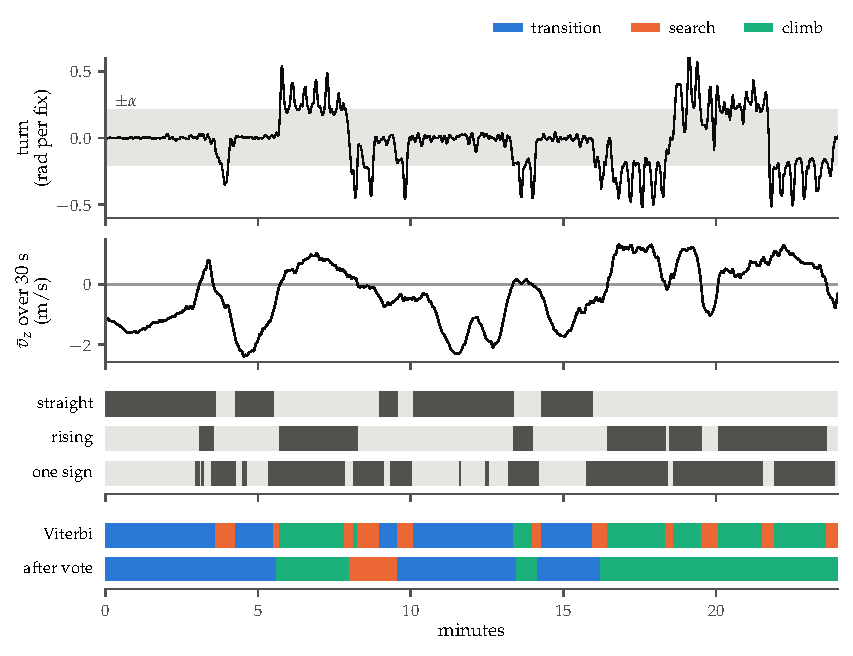
\includegraphics[width=\textwidth]{figures/features.pdf}
\caption{The features on 24 minutes of the flight of Figure~\ref{fig:flight}. From the top: the
smoothed turn, with the band $|\theta|<\alpha$ in grey; the climb rate averaged over 30~s; the
three features, dark when 1; the Viterbi path and the labels after the majority vote
(Section~\ref{sec:decoding}).}
\label{fig:features}
\end{figure}

\subsection{The straightness threshold}\label{sec:alpha}

$\alpha$ separates a turn from a wobble. Vilpellet reads it off the distribution of $|\theta|$ over
many fixes~\cite{vilpellet2026,vilpellet2025}: for paragliders and hang gliders the density decreases
from zero, first convex and then concave, and $\alpha$ is the inflection point between the two,
estimated with kernel estimates of the density and of its second derivative. He finds
$\alpha=0.2096$~rad per fix for paragliders and $0.1740$ for hang gliders ($0.10$ for sailplanes,
from a different rule). Figure~\ref{fig:alpha} shows where $\alpha$ falls on the turns of each
phase: 98\% of the transition fixes are below it, 66\% of the search fixes and 37\% of the climb
fixes.

\begin{figure}
\centering
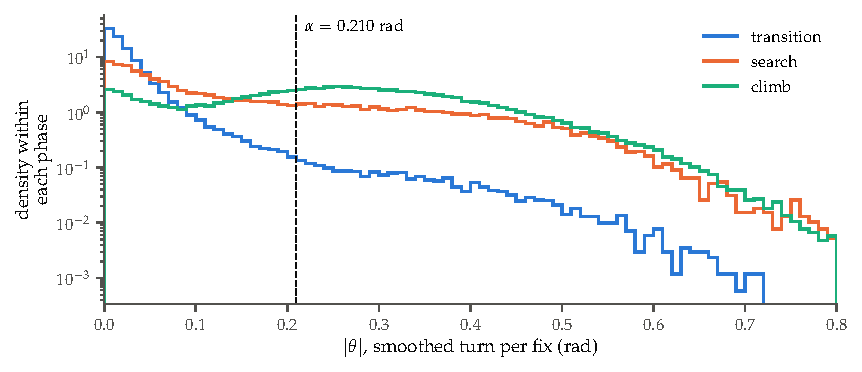
\includegraphics[width=\textwidth]{figures/turn_density.pdf}
\caption{Density of the smoothed $|\theta|$ in each phase, on 30 flights of the sample of
Section~\ref{sec:cadence}, labelled by the method; the dashed line is $\alpha$ for paragliders.}
\label{fig:alpha}
\end{figure}

\subsection{Symbols and emissions}\label{sec:emissions}

The three answers make one symbol, $x_k=4S_k+2R_k+O_k\in\{0,\dots,7\}$, and the model gives each
phase a probability for each of the eight symbols (Figure~\ref{fig:emissions}). A climb emits
almost only $(0,1,1)$, ``turning one way and rising''; a transition emits the straight symbols,
mostly $(1,0,0)$ and $(1,1,0)$; a search spreads over the other turning symbols, mostly $(0,1,0)$
and $(0,0,0)$, turning both ways with or without rising, and $(0,0,1)$, turning one way while
sinking. A straight symbol is practically impossible outside a transition, and $(0,1,1)$
practically impossible outside a climb. These symbols all but decide the phase: inside a glide a
single $(0,1,1)$ already turns the Viterbi path to climb, inside a search two in a row do, and the
majority vote of Section~\ref{sec:decoding} then removes such short runs. The HMM matters where
the symbols are ambiguous or change.

\begin{figure}
\centering
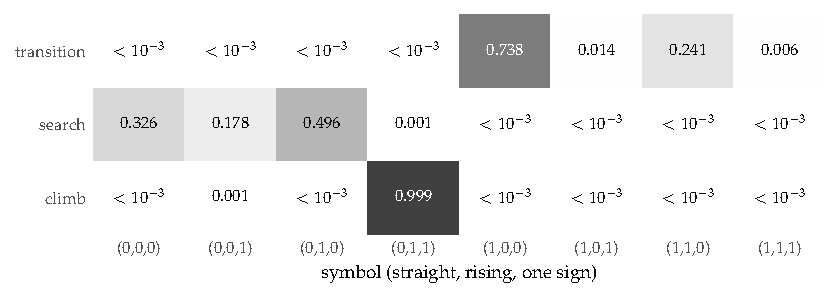
\includegraphics[width=\textwidth]{figures/emissions.pdf}
\caption{Emission probabilities $b_j(x)$ of the fitted model; each row sums to 1. Symbols are
written as (straight, rising, one sign).}
\label{fig:emissions}
\end{figure}

\subsection{Decoding and majority vote}\label{sec:decoding}

The Viterbi path~\eqref{eq:viterbi} is computed with $A$ of~\eqref{eq:A} and the initial
distribution
\[
  \nu=(0.0566,\ 0.9434,\ 6\times10^{-29}),
\]
with the scores divided by their sum at every fix; a tie goes to the phase that comes first in the
order \cl, \se, \tr. The initial probability of \tr\ is zero in practice: a piece never starts
in a transition.

The path still flickers at the changes of phase (Figure~\ref{fig:features}, ``Viterbi''). A
\emph{majority vote} follows: each fix takes the phase most frequent among the 90 fixes
$k-45,\dots,k+44$ of the path, a tie going to the phase that comes first. The vote removes the
flicker and also erases any run shorter than about 45~s, real or not.

\subsection{How the parameters were obtained}\label{sec:training}

The training script~\cite{vilpellet2025code} reads the 2019 paraglider flights from the take-offs
whose names contain Montlambert, Hilaire, Forclaz or André, keeps those with distinct
times, a mean step below 1.2~s and more than 3600 fixes, and runs five rounds of Baum--Welch from
initial values that encode Table~\ref{tab:signatures}. Each phase has one categorical law over the
eight symbols. The values in the inference script, which every later use applies unchanged, are
described there as ``a local max that is visually satisfying''. The same values serve hang gliders,
with only $\alpha$ changed. Section~\ref{sec:conflicts} lists what the code does differently from
what the paper describes.

\subsection{Which state is which}\label{sec:naming}

An HMM does not name its states (Section~\ref{sec:three}). The emissions do: the state that emits
$(0,1,1)$ is the climb and the one that emits straight symbols the transition. The training code
orders the states as thermalling, area-restricted search and commuting, consistently with the
emissions. The last line of the inference script, \texttt{regime\_map = \{0: "transition", 1:
"search", 2: "climb"\}}, swaps the first and the third. The emissions, and the climb rate,
straightness and turn sign measured in each state on five real flights~\cite{legacyguide}, show that
state 0 is the climb: the order is \cl, \se, \tr, as in this note.

\section{The paper and the code}\label{sec:conflicts}

The paper~\cite{vilpellet2026} describes the method in its appendix; the internship
report~\cite{vilpellet2025} gives the feature definitions in more detail; the code~\cite{vilpellet2025code}
is what produced the labels. Table~\ref{tab:conflicts} lists where they disagree. Each point was
checked on the code; the file and line are given where they help.

\begin{table}
\centering
\small
\renewcommand{\arraystretch}{1.15}
\begin{tabularx}{\textwidth}{@{}>{\raggedright}p{0.4cm} >{\raggedright}p{2.2cm} >{\raggedright}X >{\raggedright\arraybackslash}X@{}}
\toprule
 & topic & paper (and report) & code \\
\midrule
1 & windows & ``a rolling time window of 30 s'' & 30 \emph{fixes}; smoothing over 6 fixes, vote over 90: seconds only at 1~Hz \\ \addlinespace
2 & one-sign feature & ``sign preserved for at least 90\% of samples within the window''; the report counts all the turns of the window & at least 14 of the \emph{15 largest} $|\theta|$ of the 30 share a sign (\texttt{sliding\_}\allowbreak\texttt{window\_}\allowbreak\texttt{sign\_check}) \\ \addlinespace
3 & straight feature & ``below a prescribed threshold for at least 90\% of the window'' & more than 90\%: at least 28 of 30 instead of 27 \\ \addlinespace
4 & smoothing & not mentioned & Gaussian smoothing of the positions over 6 fixes; mean of the turn over 6 fixes \\ \addlinespace
5 & output & the Viterbi path & the Viterbi path, then a majority vote over 90 fixes (\texttt{roll\_majority}) \\ \addlinespace
6 & estimation & ``the final parameter estimates are determined entirely by the data'' (Baum--Welch) & the training model never updates $A$: the line is commented out (\texttt{hmm\_model\_}\allowbreak\texttt{bernouilli\_}\allowbreak\texttt{dependant.py}, line 222). The $A$ in use carries the marks of the constraint function \texttt{apply\_}\allowbreak\texttt{constraint}, whose call is commented out too (line 241): diagonal of \se\ at its bound $0.99$, off-diagonal entries of the \cl\ and \se\ rows in ratio exactly 2:1. Five rounds only; values kept as ``a local max that is visually satisfying'' \\ \addlinespace
7 & parameters & ``24 parameters'' & $3\times8$ emissions, $3\times3$ transitions and 3 initial values: 36 numbers, 29 free \\ \addlinespace
8 & training data & calibrated on the dataset of the paper: 49\,939 paraglider flights, 2016--2021 & 2019 flights from four Alpine take-off names; one set of parameters for every aircraft, with only $\alpha$ changed \\ \addlinespace
9 & selection & at least 1~Hz, one hour and 15~km, without spatial or temporal discontinuities & distinct times, mean step below 1.2~s, more than 3600 fixes; windows count fixes across any time gap \\ \addlinespace
10 & state names & transition, search, climb & the inference script swaps climb and transition (\texttt{regime\_map}, Section~\ref{sec:naming}) \\ \addlinespace
11 & height & in the ENU frame ``$z$ retains the physical interpretation of altitude'' & the up coordinate of the plane tangent at the first fix, below the altitude by $d^2/2R$; the climb rate loses $(d/R)\,\dot d$ (Section~\ref{sec:frame}) \\
\bottomrule
\end{tabularx}
\caption{Where the paper and the code disagree.}
\label{tab:conflicts}
\end{table}

Three facts appear in neither text: the initial probability of \tr\ is zero in practice
(Section~\ref{sec:decoding}); $\alpha$ is a per-fix angle, so its meaning changes with the logging
interval; and the scripts do not record whether $\alpha$ was estimated on the raw or on the
smoothed turn.

\begin{keypoint}{What this means for us.}
The emissions were fitted on the features of the code, so we follow the code wherever the two
disagree on the features, the smoothing and the vote (points 1--5). Point~6 means that the shipped
training script does not regenerate the shipped parameters: if the model is ever refitted, the
update of $A$ must be switched on and any constraint stated. Point~10 is a naming slip, and we name
the states from their emissions. Point~11 matters only far from the first fix of a piece, and is
one of the changes that wait for evidence (Section~\ref{sec:keep}).
\end{keypoint}

\section{What we keep, what we change}\label{sec:keep}

His segmentation already labels flights well, so we change only what running it in xc-dynamics on
every flight requires (Table~\ref{tab:keep}). The method itself, features, parameters and
decoding, stays as his code runs it.

\begin{table}
\centering
\small
\renewcommand{\arraystretch}{1.15}
\begin{tabularx}{\textwidth}{@{}>{\raggedright}p{2.3cm} >{\raggedright}X >{\raggedright}X >{\raggedright\arraybackslash}p{4.1cm}@{}}
\toprule
 & Vilpellet's code & ours & why \\
\midrule
\multicolumn{4}{@{}l}{\textit{kept}} \\
input & latitude, longitude, GNSS height of the IGC fixes & the same, after the xc-dynamics pre-processing & the pre-processing deletes bad fixes and smooths nothing, so the features see what his saw \\ \addlinespace
features & frame, smoothing, turn, climb rate, $S$, $R$, $O$, $\alpha$ (Section~\ref{sec:method}) & the same & the emissions were fitted on them \\ \addlinespace
model & emissions, $A$, $\nu$ & the same, not refitted & no labels to refit against; his labels look right \\ \addlinespace
decoding & Viterbi, then a majority vote over 90 fixes & the same & \\ \addlinespace
\multicolumn{4}{@{}l}{\textit{changed or added}} \\
unit & the whole track & one piece of the pre-processing & no window and no run crosses a split \\ \addlinespace
time & fixes as they come; windows count fixes, across gaps too & a regular 1-s grid per piece, interpolated with a cubic spline & windows mean seconds again; 2--5~s loggers become usable (Section~\ref{sec:cadence}) \\ \addlinespace
gaps & none & a gap longer than $\max(4\,\mathrm{s},2\Delta)$ ends a piece & interpolation does not bridge a hole in the track \\ \addlinespace
labels & every fix & real fixes only; interpolated seconds only feed the features & no invented fix enters a statistic \\ \addlinespace
eligibility & mean step below 1.2~s; at least 3600 fixes & any interval up to 5~s; a piece shorter than 30~s stays unlabelled & 3600 fixes selected flights for his study and is not part of the method \\ \addlinespace
state names & \texttt{regime\_map} swaps climb and transition & from the emissions & Section~\ref{sec:naming} \\ \addlinespace
\multicolumn{4}{@{}l}{\textit{left out}} \\
his advice & drop the last 10 minutes, short runs, searches not followed by a climb & not part of the labelling & they select runs for an analysis, which must say so \\
\bottomrule
\end{tabularx}
\caption{From his code to ours.}
\label{tab:keep}
\end{table}

Four changes wait for evidence. They are made only if checks on real flights show the problem:
emissions for hang gliders, which reuse those fitted on paragliders; $\alpha$ estimated again on
our data; a shorter vote, if the 90-fix majority erases real short climbs; the climb rate from
the recorded altitude, as in the frame of the thesis, instead of the height above the tangent
plane (Section~\ref{sec:frame}). The last one changes no label on the flight saved by
\texttt{cadence.py}, which stays within about 10~km of its first fix; long flights will tell.

\section{Below 1 Hz}\label{sec:cadence}

\subsection{Why everything is tied to 1 Hz}

Every number of the method counts fixes: the smoothing over 6, the windows over 30, the vote over
90, $\alpha$ in radians per fix, and $A$, which gives the probability of a change between two
consecutive fixes. On a track logged every 5~s the same code would read 30 fixes as two and a half
minutes, compare a 5-s turn with a 1-s threshold, and let phases change five times less often. His
training script keeps only tracks whose mean step is below 1.2~s; the inference script checks
nothing, and would label such a track with the numbers of 1~Hz.

There are two ways around it. One is to rescale every number to the logging interval $\Delta$:
windows of $30/\Delta$ fixes, a new $\alpha$, the matrix $A^\Delta$, a vote over $90/\Delta$ fixes.
Each of these is a new assumption to check, and at 5~s a window of six fixes leaves little to
count. The other is to bring the track to the method: interpolate it onto a regular 1-s grid and
run the method unchanged, keeping the labels of the real fixes only. We take the second, as agreed
on 20 October 2026; what remains to choose is the interpolation.

\subsection{What interpolation does to the features}

Linear interpolation joins two kept fixes with a straight segment. Between them the heading is
constant, and the whole turn of $\Delta$ seconds happens at the kept fix. After the smoothing of
Section~\ref{sec:frame} and the six-fix mean, the average turn per fix comes out right, but its
profile is spiky: a single kept fix weighs on three or four consecutive values
(Figure~\ref{fig:interpolation}). A cubic spline~\cite{deboor2001} bends between the kept fixes
and spreads the turn as the 1-Hz track does. Tremblay et al.~\cite{tremblay2006} compared the
two kinds on tracks of seabirds and seals thinned from a fine resolution: the error on the
positions hardly depended on the method, while the curvilinear ones (Bézier, Hermite, cubic
spline) gave better track lengths than straight segments. Section~\ref{sec:measurement} repeats
their design, with the labels as the quantity compared.

\begin{figure}
\centering
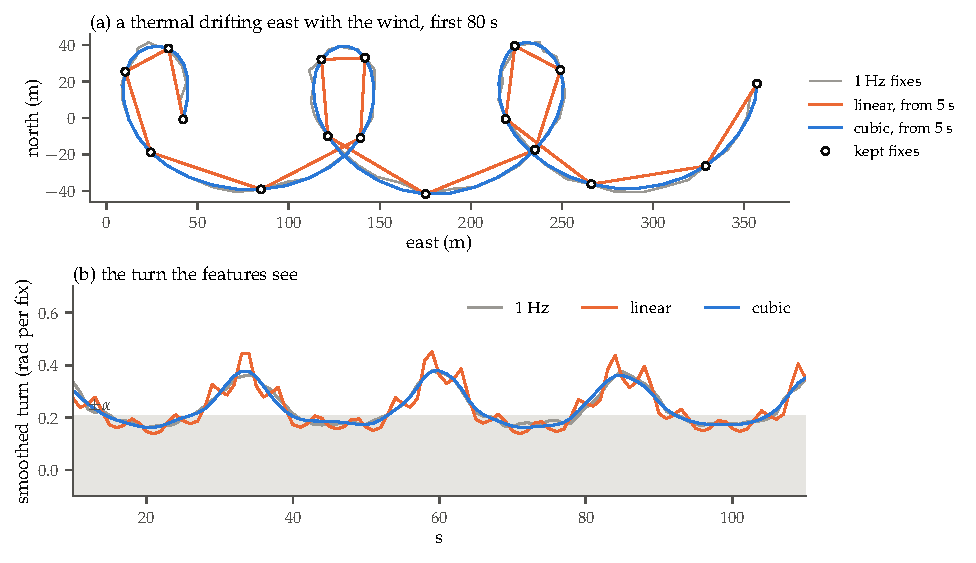
\includegraphics[width=\textwidth]{figures/interpolation.pdf}
\caption{A synthetic thermal, circles of 40~m radius every 26~s drifting east at 4~m/s, climbing at
2~m/s, with 1~m of noise on each 1-Hz fix. (a) The kept fixes, one every 5~s, joined by straight
segments and by a cubic spline. (b) The smoothed turn computed on the 1-Hz track and on the two
interpolations: the linear one is spiky around each kept fix.}
\label{fig:interpolation}
\end{figure}

Two limits follow.
\begin{itemize}
  \item \emph{Aliasing.} The change of heading between two kept fixes is known only modulo $2\pi$,
        so a change larger than $\pi$ reads as a turn the other way. On climbs logged every 5~s
        the median change between kept fixes is 1.26~rad (72\textdegree), 15\% of the changes exceed
        2~rad and 5\% exceed 2.5~rad: drifting circles and tight turns come close to $\pi$. At
        10~s the median is 2.10~rad and a third of the changes exceed 2.5~rad. In possum tracks
        thinned from 5 to 60 minutes the turning angles likewise spread towards a uniform law,
        and a two-state switching walk told the states apart less and less
        clearly~\cite{postlethwaite2013}.
  \item \emph{The one-sign feature.} Rule~\eqref{eq:O} tolerates one disagreement among the 15
        strongest turns of a window. With linear interpolation a kept fix with the wrong sign,
        from GNSS noise or from a change near $\pi$, becomes three or four strong values of the
        wrong sign and switches the feature off. The spline dilutes it.
\end{itemize}

\subsection{The measurement}\label{sec:measurement}

\paragraph{Design.} 300 paraglider flights drawn at random (seed 2026) among those logged every
second that pass the pre-processing and have at least 3600 fixes. In each piece, for
$\Delta=2,3,4,5,10$~s, we keep the fixes whose time is a multiple of $\Delta$, interpolate them onto
a 1-s grid, label, and compare the labels of the kept fixes with the labels the method gives to the
same fixes on the full 1-s piece (\texttt{cadence.py}). The reference is the method at 1~Hz: the
question is whether a coarser logger changes what the method says, and not whether the method is
right.

\paragraph{Results.} Table~\ref{tab:cadence-results} and Figure~\ref{fig:cadence}. Up to 3~s both
interpolations keep about 98--99\% of the labels. From 4~s the linear one loses climbs: at 5~s it
keeps 90.7\% of the climbing fixes and the climb share of the flight drops from 33.3\% to 31.1\%,
while the spline keeps 96.9\% and the share moves by 0.3 points. At 10~s both fail, with fewer than
six climbing fixes in ten kept. Figure~\ref{fig:cadence-example} shows the 5-s case on one flight.

\begin{table}
\centering
\small
\setlength{\tabcolsep}{5pt}
\begin{tabular}{@{}r l r r r r r r@{}}
\toprule
$\Delta$ & interp. & fixes & same label & climb kept & search kept & climb share & worst 10\% \\
\midrule
2~s & linear & 1\,683\,979 & 98.9\% & 99.0\% & 95.8\% & 33.3\% & 97.0\% \\
    & cubic  &             & 99.0\% & 99.0\% & 97.2\% & 33.3\% & 97.2\% \\ \addlinespace
3~s & linear & 1\,125\,818 & 98.2\% & 98.2\% & 92.7\% & 33.2\% & 95.6\% \\
    & cubic  &             & 98.8\% & 98.8\% & 96.1\% & 33.3\% & 96.4\% \\ \addlinespace
4~s & linear & 844\,257 & 97.1\% & 96.4\% & 89.4\% & 32.8\% & 94.1\% \\
    & cubic  &          & 98.3\% & 98.3\% & 94.1\% & 33.3\% & 96.1\% \\ \addlinespace
5~s & linear & 676\,249 & 94.8\% & 90.7\% & 86.2\% & 31.1\% & 89.3\% \\
    & cubic  &          & 97.5\% & 96.9\% & 91.3\% & 33.0\% & 94.7\% \\ \addlinespace
10~s & linear & 338\,359 & 73.2\% & 33.1\% & 81.7\% & 12.6\% & 58.7\% \\
     & cubic  &          & 81.4\% & 57.0\% & 71.6\% & 20.8\% & 69.6\% \\
\bottomrule
\end{tabular}
\caption{Labels of thinned flights against the labels of the full 1-s flights, on the kept fixes.
``Climb kept'' is the share of the fixes labelled climb at 1~Hz that are still climb; the climb
share is 33.3\% at 1~Hz; ``worst 10\%'' is the agreement that 10\% of the flights fall below.}
\label{tab:cadence-results}
\end{table}

\begin{figure}
\centering
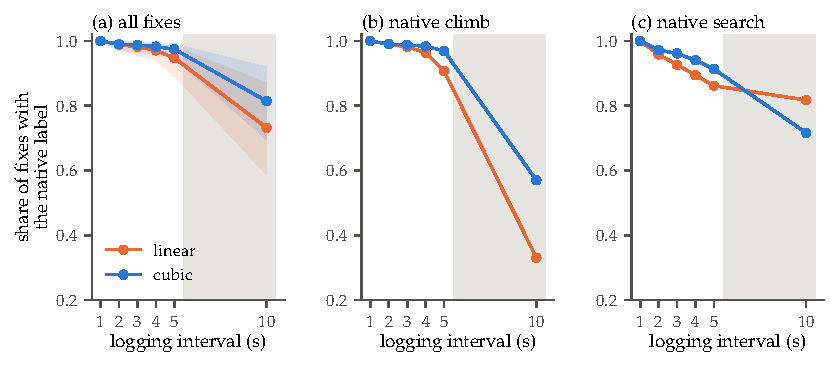
\includegraphics[width=\textwidth]{figures/cadence.pdf}
\caption{Share of the kept fixes that keep their 1-Hz label, against the logging interval: (a) all
fixes, with the band between the 10\% and 90\% of the flights; (b) fixes labelled climb at 1~Hz;
(c) fixes labelled search at 1~Hz. Grey: beyond 5~s.}
\label{fig:cadence}
\end{figure}

\begin{figure}
\centering
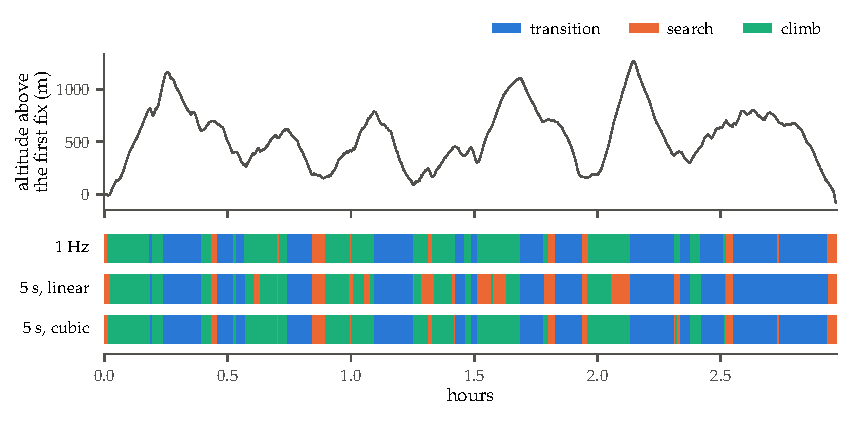
\includegraphics[width=\textwidth]{figures/cadence_example.pdf}
\caption{The flight of Figure~\ref{fig:flight}, labelled at 1~Hz and from one fix every 5~s. With
linear interpolation several climbs turn into searches; with the spline they come back. This flight
is in the worst tenth of the sample for the linear case: it keeps 87\% of its labels against 98.5\%
with the spline.}
\label{fig:cadence-example}
\end{figure}

\paragraph{Mechanism.} On 40 of the flights (\texttt{mechanism.py}), 5.6\% of the climbing fixes
change their symbol from $(0,1,1)$ to $(0,1,0)$ at 5~s with linear interpolation, against 1.2\%
with the spline: the one-sign feature is the one that fails. The share of climbing windows with at
least two strong turns of the minority sign grows from 8.4\% at 1~Hz to 12.9\% with linear
interpolation, and stays at 8.9\% with the spline.

\subsection{Verdict}

\begin{keypoint}{Up to one fix every 5 seconds: yes, with a cubic spline.}
Interpolating each piece onto a 1-s grid with a cubic spline and running the method unchanged
reproduces the 1-Hz labels on 99.0\% of the fixes at 2~s and 97.5\% at 5~s, and keeps the share of
each phase within half a point. Linear interpolation is enough up to 3~s and loses climbs from 4~s
on. At 10~s neither works, because the turns between two fixes reach $\pi$. Flights logged every
more than 5~s stay unlabelled: those at 10~s alone are 2.4\% of the paragliders and 15.2\% of the
hang gliders (Table~\ref{tab:cadence}).
\end{keypoint}

One caveat. Thinning a 1-Hz track keeps its receiver: a logger that records every 5~s may average
or filter its positions, and its errors are those of its own receiver. A visual check on a few
flights logged natively every 5~s, before using them, settles it.

\section{Implementation in xc-dynamics}\label{sec:implementation}

The plan agreed on 20 October 2026, with the interpolation fixed by Section~\ref{sec:cadence}. The
rewrite in this folder, \texttt{phases.py}, is the reference to test against; the code of
xc-dynamics is written there from scratch, as for every lab result.

\begin{enumerate}
  \item \textbf{An area \texttt{phases}} (``segment'' already names a piece of a split flight),
        with its source, scripts, configuration, tests and reference page, named like the other
        areas.
  \item \textbf{One piece at a time} (Figure~\ref{fig:overview}): the fixes of one
        pre-processing segment, cut again wherever a gap exceeds $\max(4\,\mathrm{s},2\Delta)$;
        a piece logged every more than 5~s, or shorter than 30~s, stays unlabelled.
  \item \textbf{A regular 1-s grid} through a cubic spline of $(e,n,u)$ over the real fixes of the
        piece.
  \item \textbf{The method of Section~\ref{sec:method}} on the grid, then the labels of the real
        fixes only.
  \item \textbf{Storage as runs}: one row per run of one phase (flight, segment, phase, first and
        last time, number of fixes, whether a cut or the end of the piece censors it), written
        in one pass over the whole archive.
\end{enumerate}

\paragraph{Configuration.} Every constant goes in \texttt{configs/phases.yaml}, a sketch of which
follows; the fitted values are those of Appendix~\ref{app:parameters}.
\begin{verbatim}
grid:
  min_gap_s: 4.0          # a longer gap ends a piece,
  gap_steps: 2            # or two logging steps if longer
  max_interval_s: 5.0     # coarser loggers stay unlabelled
  interpolation: cubic
features:
  smoothing_fixes: 6      # Gaussian, standard deviation one fix
  turn_mean_fixes: 6
  window_fixes: 30
  beta: 0.9
  alpha_rad: {para: 0.20960958, hang: 0.17398039}
decoding:
  vote_fixes: 90
model:                    # Vilpellet's fitted values
  states: [climb, search, transition]
  initial: [...]
  transition: [...]
  emission: [...]
\end{verbatim}

\paragraph{Tests.} The same labels as \texttt{phases.py}, and through it as the reference script, on
synthetic tracks with a glide, a thermal and a search; the small example of
Section~\ref{sec:toy}; and, when the disk is mounted, the cadence check of
Section~\ref{sec:cadence} on a few flights.

\paragraph{After that.} Visual checks on a few flights of each logging interval and of each
discipline, and only then the changes of Section~\ref{sec:keep} that wait for evidence.

\appendix
\section{The fitted parameters}\label{app:parameters}

The values of the inference script~\cite{vilpellet2025code}, in the order \cl, \se, \tr, which is
the order of its states (Section~\ref{sec:naming}).

\begin{center}
\small
\begin{tabular}{@{}l l l l@{}}
\toprule
symbol & \cl & \se & \tr \\
\midrule
0 $(0,0,0)$ & $1.54243294\times10^{-11}$ & $3.25680580\times10^{-1}$ & $6.93534587\times10^{-6}$ \\
1 $(0,0,1)$ & $5.07106916\times10^{-4}$ & $1.77503496\times10^{-1}$ & $1.04473011\times10^{-8}$ \\
2 $(0,1,0)$ & $8.72065952\times10^{-5}$ & $4.95899060\times10^{-1}$ & $2.91554932\times10^{-6}$ \\
3 $(0,1,1)$ & $9.98979845\times10^{-1}$ & $7.21547291\times10^{-4}$ & $1.93493842\times10^{-10}$ \\
4 $(1,0,0)$ & $8.52234426\times10^{-21}$ & $6.96932383\times10^{-5}$ & $7.38362033\times10^{-1}$ \\
5 $(1,0,1)$ & $1.25568196\times10^{-12}$ & $1.93093305\times10^{-5}$ & $1.40643862\times10^{-2}$ \\
6 $(1,1,0)$ & $7.85199401\times10^{-13}$ & $1.06025552\times10^{-4}$ & $2.41340621\times10^{-1}$ \\
7 $(1,1,1)$ & $4.25841826\times10^{-4}$ & $2.89805651\times10^{-7}$ & $6.22309818\times10^{-3}$ \\
\midrule
initial $\nu$ & $5.66075578\times10^{-2}$ & $9.43392442\times10^{-1}$ & $5.88699965\times10^{-29}$ \\
\bottomrule
\end{tabular}
\end{center}
Emission probabilities $b_j(x)$, one column per phase, and the initial distribution. The symbol is
written as (straight, rising, one sign).

\[
  A=\begin{pmatrix}
    0.98961359 & 0.00346214 & 0.00692427\\
    0.00666667 & 0.99000000 & 0.00333333\\
    0.00099934 & 0.00712054 & 0.99188012
  \end{pmatrix},
\]
$\alpha=0.20960958$~rad per fix for paragliders and $0.17398039$ for hang gliders.
Windows: smoothing 6 fixes (Gaussian, standard deviation one fix), turn mean 6, features 30
($\beta=0.9$), vote 90.

\begin{thebibliography}{99}
\small

\bibitem{vilpellet2026} J. Vilpellet, A. Darmon, M. Benzaquen. From random walks to thermal rides:
universal anomalous transport in soaring flights. arXiv:2601.01293, 2026. Appendix, ``Flight phase
segmentation''.

\bibitem{vilpellet2025} J. Vilpellet. \emph{Micrometeorology and optimal exploration--exploitation}.
Internship report, EconophysiX and Université Paris Dauphine--PSL, 29 September 2025. Sections 3.2
and 4.

\bibitem{vilpellet2025code} J. Vilpellet. \texttt{package\_python\_econophysix}, unpublished code,
2025: \texttt{scripts/hmm/} (features, models, training) and
\texttt{flight\_phase\_inference\_minimal.py} (inference with the fitted values, December 2025).

\bibitem{legacyguide} M. Di Sante. The Vilpellet segmenter. \texttt{docs/guide/vilpellet-segmentation.md}
of soaring-anomalous-transport, tag \texttt{legacy-final}: the measured climb rate, straightness and
turn sign of each state on five flights.

\bibitem{rabiner1989} L. R. Rabiner. A tutorial on hidden Markov models and selected applications in
speech recognition. \emph{Proceedings of the IEEE} 77(2):257--286, 1989.

\bibitem{zucchini2016} W. Zucchini, I. L. MacDonald, R. Langrock. \emph{Hidden Markov Models for Time
Series: An Introduction Using R}, 2nd edition. CRC Press, 2016.

\bibitem{langrock2012} R. Langrock, R. King, J. Matthiopoulos, L. Thomas, D. Fortin, J. M. Morales.
Flexible and practical modeling of animal telemetry data: hidden Markov models and extensions.
\emph{Ecology} 93(11):2336--2342, 2012.

\bibitem{michelot2016} T. Michelot, R. Langrock, T. A. Patterson. moveHMM: an R package for the
statistical modelling of animal movement data using hidden Markov models. \emph{Methods in Ecology
and Evolution} 7(11):1308--1315, 2016.

\bibitem{viterbi1967} A. J. Viterbi. Error bounds for convolutional codes and an asymptotically
optimum decoding algorithm. \emph{IEEE Transactions on Information Theory} 13(2):260--269, 1967.

\bibitem{forney1973} G. D. Forney. The Viterbi algorithm. \emph{Proceedings of the IEEE}
61(3):268--278, 1973.

\bibitem{baum1970} L. E. Baum, T. Petrie, G. Soules, N. Weiss. A maximization technique occurring in
the statistical analysis of probabilistic functions of Markov chains. \emph{The Annals of
Mathematical Statistics} 41(1):164--171, 1970.

\bibitem{tremblay2006} Y. Tremblay, S. A. Shaffer, S. L. Fowler, C. E. Kuhn, B. I. McDonald,
M. J. Weise, C.-A. Bost, H. Weimerskirch, D. E. Crocker, M. E. Goebel, D. P. Costa. Interpolation
of animal tracking data in a fluid environment. \emph{Journal of Experimental Biology}
209(1):128--140, 2006.

\bibitem{postlethwaite2013} C. M. Postlethwaite, T. E. Dennis. Effects of temporal resolution on an
inferential model of animal movement. \emph{PLoS ONE} 8(5):e57640, 2013.

\bibitem{deboor2001} C. de Boor. \emph{A Practical Guide to Splines}, revised edition. Springer,
2001.

\end{thebibliography}


\end{document}
